\documentclass[border=5pt]{standalone}
\usepackage[T1]{fontenc}
\usepackage{lmodern}
\usepackage{pgfplots}
\usepgfplotslibrary{groupplots}
\pgfplotsset{compat=1.18}
\begin{document}\sffamily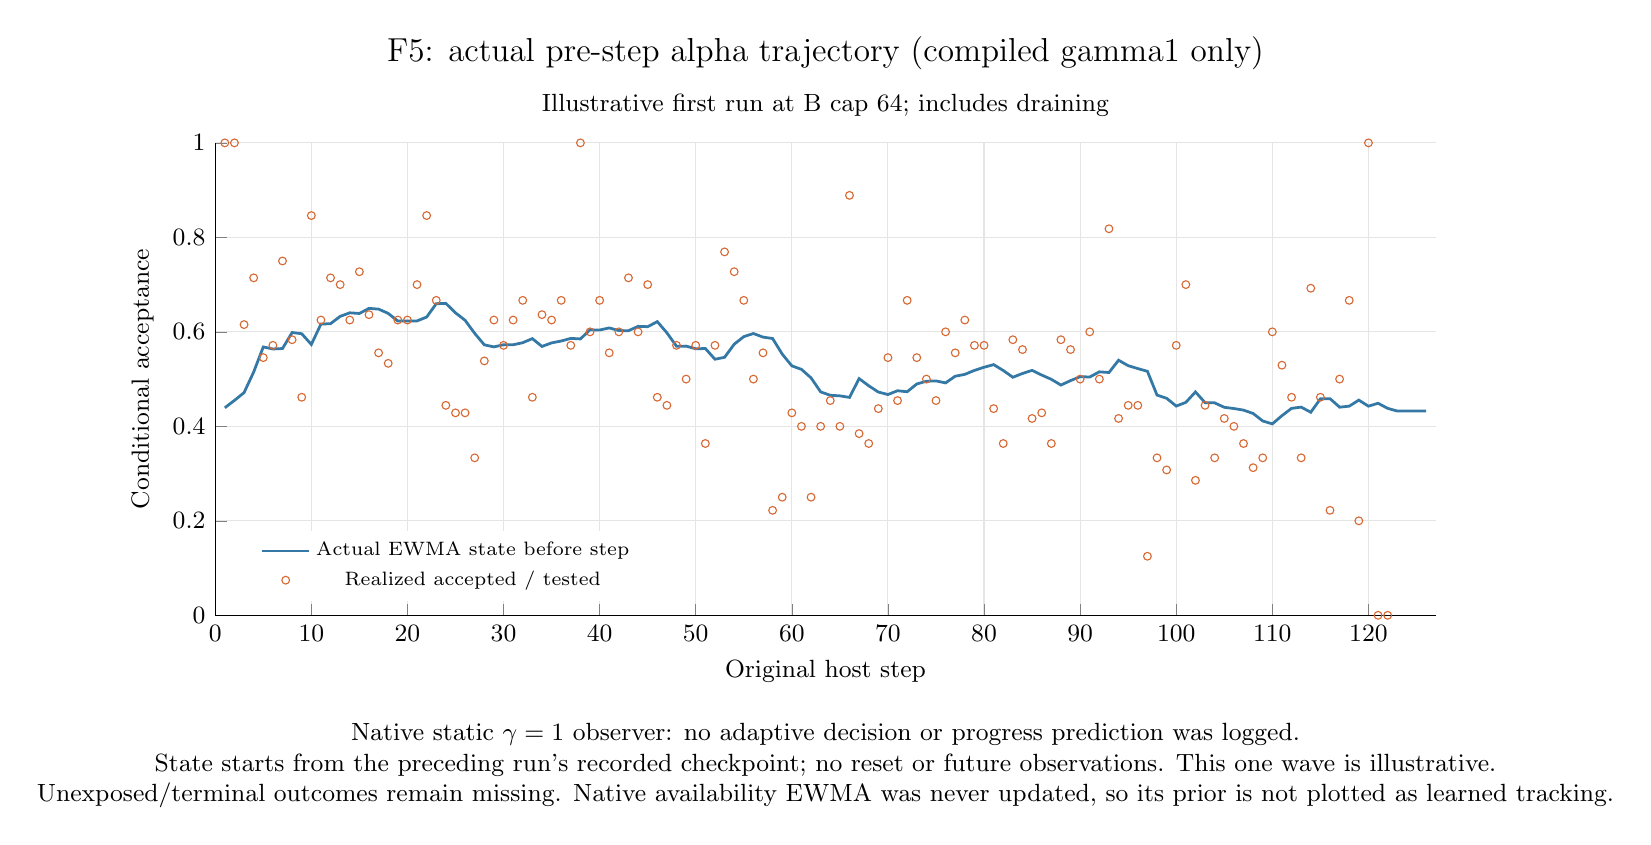
\begin{tikzpicture}
\definecolor{cal}{HTML}{3478A5}\definecolor{test}{HTML}{D76832}\definecolor{profile}{HTML}{3B8A5A}
\begin{groupplot}[group style={group size=1 by 1,horizontal sep=1.9cm},width=15.5cm,height=6.0cm,scale only axis,axis lines*=left,grid=major,grid style={gray!20},tick label style={font=\small},label style={font=\small},title style={font=\small},legend style={font=\scriptsize,draw=none},unbounded coords=jump]
\nextgroupplot[title={Illustrative first run at B cap 64; includes draining},xlabel={Original host step},ylabel={Conditional acceptance},xmin=0,xmax=127,ymin=0,ymax=1,legend pos=south west]
\addplot[color=cal,line width=1pt] coordinates {(1,0.439247788071) (2,0.454914507866) (3,0.471326163272) (4,0.514988397965) (5,0.568030501924) (6,0.563773990963) (7,0.564674404897) (8,0.59859744176) (9,0.596017653771) (10,0.573284299175) (11,0.616432883589) (12,0.617268799417) (13,0.632740016295) (14,0.640296291661) (15,0.638907469575) (16,0.649671811699) (17,0.64808526972) (18,0.639037661911) (19,0.622831729002) (20,0.62301231537) (21,0.623180675432) (22,0.631266554065) (23,0.659626198998) (24,0.660275066879) (25,0.640226424217) (26,0.624498232737) (27,0.596729532499) (28,0.572515736096) (29,0.568137347676) (30,0.572732301358) (31,0.572637336795) (32,0.577070617325) (33,0.585645210856) (34,0.569120865614) (35,0.576601857737) (36,0.580594034031) (37,0.586130000147) (38,0.584998606858) (39,0.604331844795) (40,0.603835509051) (41,0.608294315226) (42,0.602716377655) (43,0.602402652284) (44,0.611624567687) (45,0.610910821662) (46,0.62160706561) (47,0.597950119709) (48,0.569512909817) (49,0.569777273085) (50,0.564155948192) (51,0.564684189538) (52,0.542056634421) (53,0.546089564414) (54,0.573778240786) (55,0.589814398023) (56,0.596480421651) (57,0.58886739138) (58,0.585876685162) (59,0.552890975314) (60,0.527987121556) (61,0.520628398742) (62,0.502554461555) (63,0.47287162125) (64,0.465719707374) (65,0.464522877545) (66,0.461211694981) (67,0.501020885709) (68,0.485891156582) (69,0.472578619366) (70,0.467329096542) (71,0.475343877109) (72,0.473215705009) (73,0.489679343576) (74,0.495457710415) (75,0.496109174528) (76,0.492005148584) (77,0.506059325773) (78,0.510010719092) (79,0.518414616865) (80,0.525010939939) (81,0.530648796609) (82,0.518201821301) (83,0.503885932768) (84,0.511904976386) (85,0.51848648118) (86,0.508528500818) (87,0.499532244061) (88,0.487377617733) (89,0.496762970661) (90,0.505082859888) (91,0.504456202862) (92,0.515329975046) (93,0.513921611662) (94,0.539955575538) (95,0.52837024862) (96,0.522275497905) (97,0.516464244204) (98,0.466149362611) (99,0.459398072914) (100,0.442857494478) (101,0.450730849912) (102,0.472813840924) (103,0.450152865204) (104,0.449698338768) (105,0.440240188376) (106,0.437706660659) (107,0.434293982318) (108,0.427256430865) (109,0.411345225821) (110,0.405124025339) (111,0.422590499203) (112,0.438056771123) (113,0.440629069004) (114,0.429791625319) (115,0.458248645438) (116,0.45860229397) (117,0.440548714462) (118,0.442709492249) (119,0.455500977109) (120,0.442667513982) (121,0.44881974226) (122,0.43807359841) (123,0.432322954345) (124,0.432322954345) (125,0.432322954345) (126,0.432322954345)};
\addlegendentry{Actual EWMA state before step}
\addplot[only marks,color=test,mark=o,mark size=1.4pt] coordinates {(1,1) (2,1) (3,0.615384615385) (4,0.714285714286) (5,0.545454545455) (6,0.571428571429) (7,0.75) (8,0.583333333333) (9,0.461538461538) (10,0.846153846154) (11,0.625) (12,0.714285714286) (13,0.7) (14,0.625) (15,0.727272727273) (16,0.636363636364) (17,0.555555555556) (18,0.533333333333) (19,0.625) (20,0.625) (21,0.7) (22,0.846153846154) (23,0.666666666667) (24,0.444444444444) (25,0.428571428571) (26,0.428571428571) (27,0.333333333333) (28,0.538461538462) (29,0.625) (30,0.571428571429) (31,0.625) (32,0.666666666667) (33,0.461538461538) (34,0.636363636364) (35,0.625) (36,0.666666666667) (37,0.571428571429) (38,1) (39,0.6) (40,0.666666666667) (41,0.555555555556) (42,0.6) (43,0.714285714286) (44,0.6) (45,0.7) (46,0.461538461538) (47,0.444444444444) (48,0.571428571429) (49,0.5) (50,0.571428571429) (51,0.363636363636) (52,0.571428571429) (53,0.769230769231) (54,0.727272727273) (55,0.666666666667) (56,0.5) (57,0.555555555556) (58,0.222222222222) (59,0.25) (60,0.428571428571) (61,0.4) (62,0.25) (63,0.4) (64,0.454545454545) (65,0.4) (66,0.888888888889) (67,0.384615384615) (68,0.363636363636) (69,0.4375) (70,0.545454545455) (71,0.454545454545) (72,0.666666666667) (73,0.545454545455) (74,0.5) (75,0.454545454545) (76,0.6) (77,0.555555555556) (78,0.625) (79,0.571428571429) (80,0.571428571429) (81,0.4375) (82,0.363636363636) (83,0.583333333333) (84,0.5625) (85,0.416666666667) (86,0.428571428571) (87,0.363636363636) (88,0.583333333333) (89,0.5625) (90,0.5) (91,0.6) (92,0.5) (93,0.818181818182) (94,0.416666666667) (95,0.444444444444) (96,0.444444444444) (97,0.125) (98,0.333333333333) (99,0.307692307692) (100,0.571428571429) (101,0.7) (102,0.285714285714) (103,0.444444444444) (104,0.333333333333) (105,0.416666666667) (106,0.4) (107,0.363636363636) (108,0.3125) (109,0.333333333333) (110,0.6) (111,0.529411764706) (112,0.461538461538) (113,0.333333333333) (114,0.692307692308) (115,0.461538461538) (116,0.222222222222) (117,0.5) (118,0.666666666667) (119,0.2) (120,1) (121,0) (122,0)};
\addlegendentry{Realized accepted / tested}
\end{groupplot}
\path (group c1r1.north west) -- node[above=0.8cm,font=\large] {F5: actual pre-step alpha trajectory (compiled gamma1 only)} (group c1r1.north east);
\path (group c1r1.south west) -- node[below=1.25cm,align=center,font=\small] {Native static $\gamma=1$ observer: no adaptive decision or progress prediction was logged.\\State starts from the preceding run's recorded checkpoint; no reset or future observations. This one wave is illustrative.\\Unexposed/terminal outcomes remain missing. Native availability EWMA was never updated, so its prior is not plotted as learned tracking.} (group c1r1.south east);
\end{tikzpicture}\end{document}
